\chapter{Thermometry of an ultracold Fermi gas}
\label{ch:idealfermigas}
The purpose of the camera is to measure distributions of atoms from which important physical quantities can be extracted. Dense atomic clouds consisting of Lithium and Caesium, the improvement of the resolution in the whole imaging setup now allows to explore new features that could not be detected before. As an example, the thermometry of an ultracold ideal Fermi Gases will be discussed in this chapter. At very low temperatures, the gas undergoes a phase transition from thermal into a degenerate state. This is reflected in the density distribution, which differs from a gaussian profile that one expects for a thermal gas.

These changes are small, nevertheless, they can be detected with the new setup. Therefore, this chapter starts with a brief introduction to absorption imaging in \refSec{absim}, which is used to image the atoms. Afterwards, the density distribution of ultracold, ideal Fermi gases in harmonic confinement are explained in \refSec{densdistrfermi}.
Finally, in \refSec{fermiexperiment}, the performed experiment with an ultracold gas of Li atoms and their analysis are presented.

\section{Absorption imaging}
\label{sec:absim}
In order to find microscopic properties of atoms, or assembles of atoms, it is necessary to look at the atoms themselves. This is commonly accomplished using either fluorescence or absorption imaging\cite{Murmann2011}. In both cases, a laser beam is pointed at an atomic cloud, that is cooled and confined in a trap. In fluorescence imaging, the scattered light is collected, typically in a direction that is different than the illuminating beam.
The intensity from the light reaching the detector is not very high, since it is radiated in all directions. Therefore, long exposure times are required during which atoms can move and the information about the initial density and energy distribution is lost. Nevertheless, this approach is useful for single- and few-atom detection.

In contrast, in absorption imaging\cite{helmrich2013}, the transmitted intensity of an imaging beam is recorded. Without atoms, one would detect the beam profile of the laser beam. With atoms, a shadow is visible due to the atoms "blocking" the light. This is accomplished, by correctly tuning the laser to a resonance frequency of the atoms, which enables them to absorb the light, exciting them to a higher state. Through spontaneous emission, the atoms will decay, making it possible to excite them once again. This method works well, when the "signal" from the absorbed light is significantly larger compared to the noise sources, and the atomic transition used for imaging is "closed", i.e. the excited atoms decay only into the imaging state.

In order to extract physical properties of the atoms after they have been illuminated, a quantity called optical density $OD$ is found in the absorption profile, which has an exponential dependency to the intensity reaching the CCD. From the optical density, one can conclude for example atomic distribution and atom numbers.
This is put into equations as follows:\cite{Murmann2011}
\begin{equation}
I_{CCD} = I_0 e^{-OD} + I_{back},
\end{equation}
which is decreasing from the initial intensity $I_0$ as the light is scattered by atoms. The intensity $I_{back}$ describes the background signal, that is found when the CCD is not being illuminated by a laser such as readout noise, dark noise or stray photon light. All the features of atoms are contained in the optical density, therefore in order to extract that, a background frame is subtracted from the absorption image and the laser profile divided, leaving
\begin{equation}
\frac{I_{CCD} - I_{back}}{I_0} = e^{-OD}.
\end{equation}
The laser intensity $I_0$ is measured in a separate frame, containing the laser intensiy $I_0' = I_0 + I_{back}$ and also the background $I_{back}$. Finally, for each pixel of the CCD detector, the equation yields
\begin{equation}
\frac{I_{CCD} - I_{back}}{I_0' - I_{back}} = e^{-OD}.
\end{equation}

From the resulting distribution of optical density, one can now extract, for example, atom density distributions, atom numbers or excitation rates.

\section{Density distribution of an ideal Fermi gas}
\label{sec:densdistrfermi}

An ideal Fermi gas consists of only one spin component. This way, each energy level in a harmonic potential up to the chemical potential $\mu$ is occupied by one or zero atoms, so that the Fermions do not interact with each other. This leads to a new distribution of the atoms, which differs from the common Maxwell-Boltzmann distribution of thermal clouds.

The fermionic cloud can be characterized by the degeneracy parameter $T/T_F$. For values $T/T_F \gg 1$ the gas is then called thermal and will follow Maxwell-Boltzmann statistics. The cloud is called degenerate for $T/T_F \ll 1$ and the density profile will be a Fermi distribution. This is analogue to introducing a parameter $q=\frac{\mu}{k_BT}$ with the Boltzmann constant $k_B$ and the Temperature $T$, which is negative in the thermal and positive in the degenerate regime.

In order to find out if the cloud is thermal or degenerate, one can fit a distribution, that interpolates between both regimes. The following derivations can be found in \cite{Ketterle2008}.

In the Maxwell-Boltzmann distribution, the radius is defined by
\begin{equation}
\sigma _i = \sqrt{\frac{2k_BT}{mw_i^2}},
\end{equation}
where $m$ is the mass of Lithium and $w_i$ is the trapping frequency in the $i=\{x,y,z\}$ direction of the radius. Due to the alignment of the dipole trap, the cloud will not have a spherical shape and will therefore have different radii\cite{Heck2012}.

In the degenerate regime however, the atom density is best described by a Thomas-Fermi distribution with the Fermi radius
\begin{equation}
R_{Fi} = \sqrt{\frac{2E_F}{mw_i^2}},
\end{equation}
where $E_F=\hbar \bar{w} (6N)^{1/3}$ is the Fermi energy ($N$ being the number of atoms and $\bar{w}=(w_1 w_2 w_3)^{1/3}$ the trapping frequency).

Therefore a unified radius,
\begin{equation}
R_i^2 = \frac{2k_BT}{mw_i^2}f( e^{q}),
\end{equation}
can be used, with the previously declared shape parameter $q$. It smoothly interpolates between the two regimes and is used in fitting the atom density distributions.
The interpolation function $f(x)$ is
\begin{equation}
f(x) = \frac{Li_1(-x)}{Li_0(-x)} = \frac{1+x}{x} ln(1+x),
\end{equation}
where $Li_n$ is the n-th order polylogarithm and can be defined as
\begin{equation}
Li_s(z) = \sum_{k=1}^{\infty} \frac{z^k}{k^s}.
\end{equation}

In our case, we integrate over all but one axes, and therefore the fitting function for the atom density distribution yields
\begin{equation}
\label{eq:n1d}
n_{1D}(x) = n_{1D,0}\frac{Li_{5/2}\left( \pm \mathrm{exp}\left[ q-\frac{x^2}{R_x^2}f(e^q)\right] \right)}{Li_{5/2}(\pm e^q)}.
\end{equation}
During fitting, the shape parameter $q=\frac{\mu}{k_B T}$ is extracted, which describes the ratio between chemical potential and thermal energy of the gas.

In order to calculate the degeneracy parameter $T/T_F$, the value of $q$ is inserted into the equation:
\begin{equation}
\label{eq:tovertf}
\frac{T}{T_F} = \left[ -6 Li_3(-e^q) \right]^{-1/3}.
\end{equation}

As the camera only has a finite resolution, the cloud can be released and imaged after a short time. At the time of the acqusition, the gas will have expanded, although the distribution is approximately the same. During expansion of the cloud, the temperature, which is dependent on the radius, will not change. Therefore, the radius is contracted in order to receive the radius of the inital distribution by
\begin{equation}
R_{0,i} = \frac{R_{i}}{\sqrt{1+ w_i^2}},
\end{equation}
which can then be used to calculate the temperature of the cloud using
\begin{equation}
\label{eq:temp}
k_BT = \frac{1}{2} mw_i^2 \frac{R_i^2}{1+w_i^2t^2}\frac{1}{f(e^q)}.
\end{equation}


	
\section{Preparation and imaging of an ultracold Fermi gas}
\label{sec:fermiexperiment}

As seen before, from an ideal Fermi gas, one can deduce the temperature and Fermi temperature of a gas.
In order to implement ideal Fermi gases, Lithium was prepared in an optical dipole trap. The power was ramped down several times at the Feshbach resonance $B=\SI{896}{\gauss}$, until only a fraction of the atoms remained. The spin-down atoms received a short laser pulse, so that the cloud only consisted of spin-up $^6$Li.

\pltCustom{
	\begin{center}
		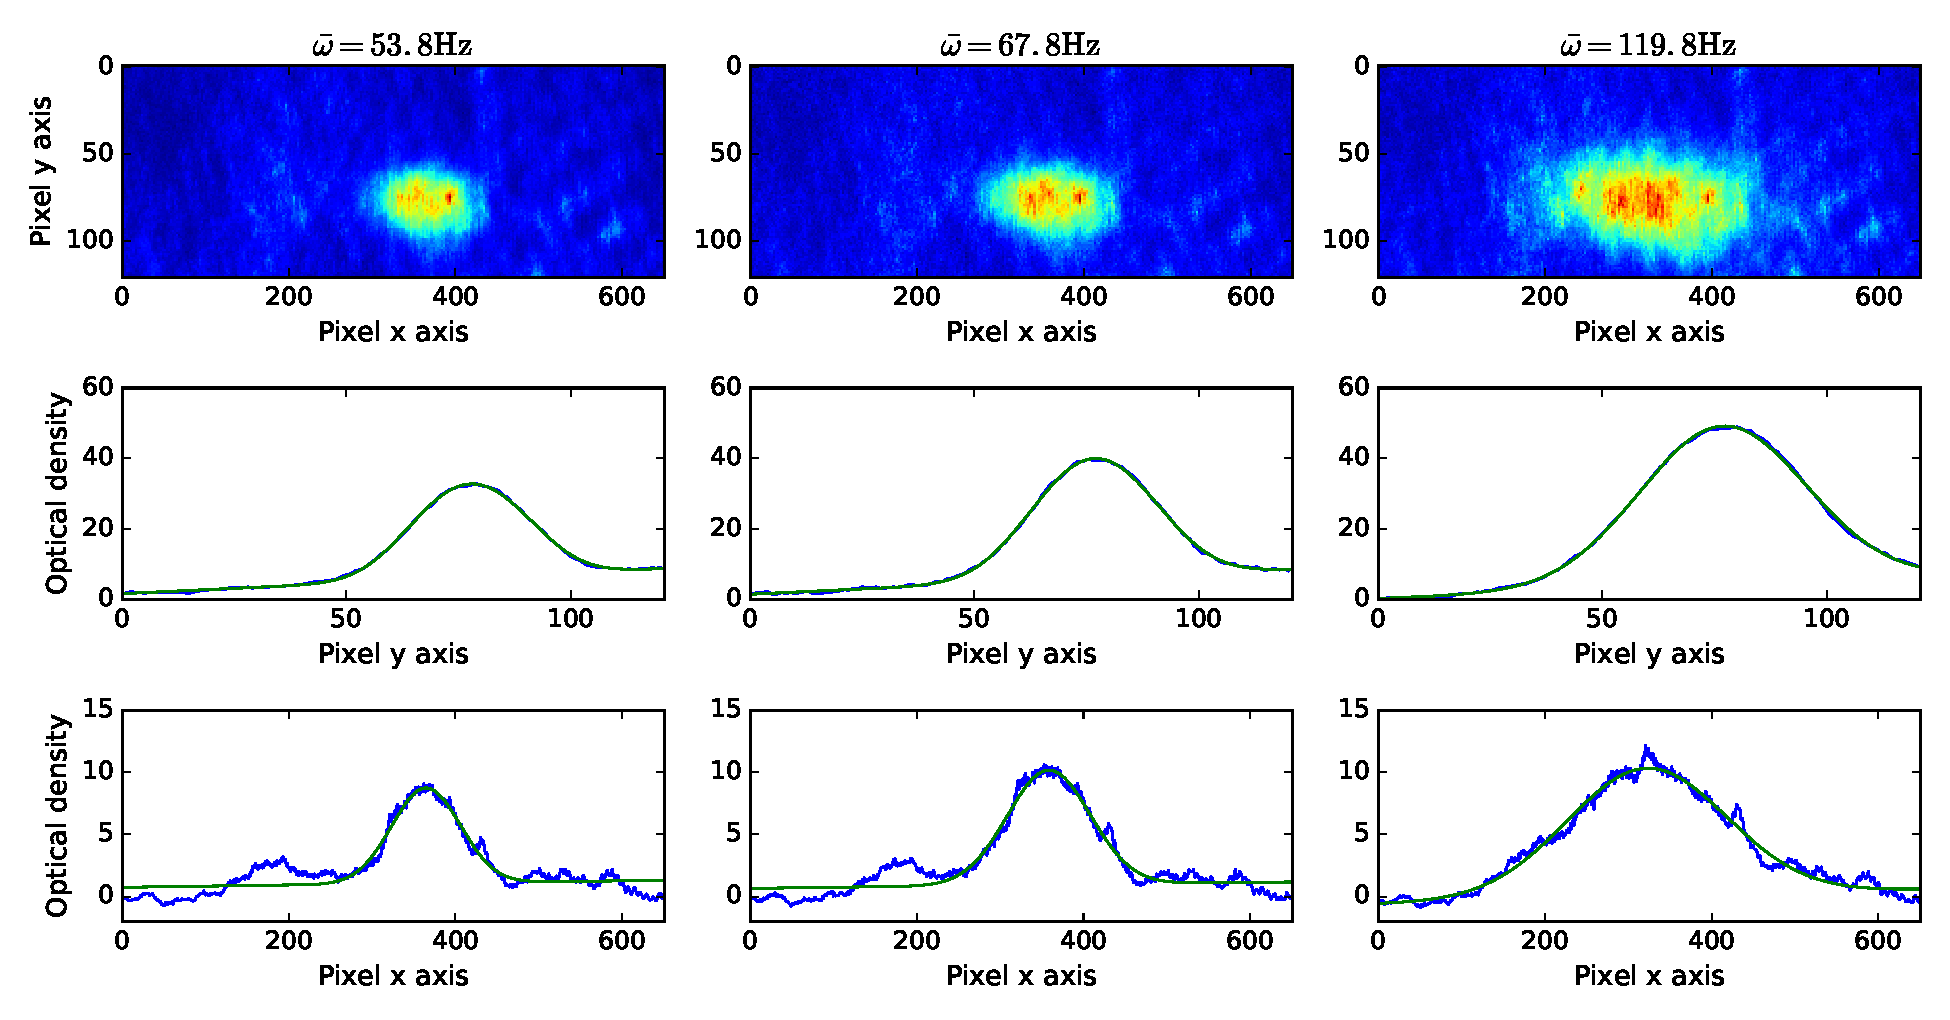
\includegraphics[width=1\textwidth]{drafts/fermi_fit.pdf}
	\end{center}
	\begin{textblock}{2}(0.75,-4.7)
		\textbf{a.}
	\end{textblock}
	\begin{textblock}{2}(4.55,-4.7)
		\textbf{b.}
	\end{textblock}
	\begin{textblock}{2}(8.35,-4.7)
		\textbf{c.}
	\end{textblock}
}{fermi_fit}{Fitting the fermi distribution to an ideal Fermi gas}{In order to find the physical properties of a fermionic cloud, they were imaged at three different trap depths which correspond to the $\bar{\omega} = (\omega_x \omega_y \omega_z)^{1/3}$, where $w_i$ is the trap frequency in the corresponding axis. As of the writing of this thesis, the imaging system was not yet well aligned in the x-Direction, therefore the data does not represent the theory well. The results of the fits are given in Table \ref{tab:fermi_fit}.}

The measurement was executed for three different powers of the laser beam. The atoms were imaged after a short time of flight of \SI{1}{\milli\second}. In order to fit the function \refEq{n1d}, the absorption image yielding the optical density as seen in \refFig{fermi_fit} was integrated over one axis, giving a one dimensional distribution for the atoms.

As the imaging is not properly optimized at this point, the distribution in the horizontal (x-axis) direction does not represent the theory well, even after averaging over several acquisitions. This problem could not be resolved due to timing constrictions, therefore the fit parameters were extracted solely from the vertical direction.

On the vertical axis, a common systematic error was a small peak for high values, which did not correspond to the atoms and is probably due to the lenses, which are not properly aligned. This was excluded from the fit. Due to the alignment in the x-Direction, the measurement could not be included, as the fragments disturbed the data too much.
\begin{table}
	\begin{center}
		\begin{tabular}{M{1cm}!M{4cm}|M{4cm}|M{4cm}N}
			& $\bar{\omega}=\SI{53.8}{\hertz}$ & $\bar{\omega}=\SI{67.8}{\hertz}$ & $\bar{\omega}=\SI{119.8}{\hertz}$ & \\[7pt]
			\thickhline
			$n_{1D}$ & $25.6\pm0.1$ & $34.07\pm0.13$ & $44.98\pm0.24$ & \\ [7pt]
			\hline
			$q$ & $1.87\pm0.35$ & $1.08\pm0.34$ & $-2.0\pm1.85$ & \\[7pt]
			\hline
			$R_y$ & $23.9\pm0.72$ & $23.80\pm0.75$ & $26.79\pm1.06$ & \\[7pt]
			\hline
			$T$ & $(5.92\pm0.55)*10^{-8}$ & $(7.43\pm0.14)*10^{-7}$ & $(1.23\pm0.25)*10^{-6}$ & \\[7pt]
			\hline
			$T/T_F$ & $0.34$ & $0.42$ & $1.01$ & \\[7pt]
		\end{tabular}
	\end{center}
	\setCaption{Fit parameters for various trap depths}{The Fermions were fitted using \refEq{n1d}, where the parameter $n_{1D}$ describes the amplitude of the peak. $q$ is a shape parameter, which is negative if the cloud is thermal or positive if the cloud is degenerate. $R_y$ is then the clouds radius similar as the radius can be described in a gaussian distribution which is in units of pixels and can be calculated in natural units using the pixel size (\SI{13}{\micro\meter}) and the magnification ($7.5$).}
	\label{tab:fermi_fit}
\end{table}

In order to properly fit \refEq{n1d}, a linear function had to be added, as there was a constrant gradient on the chip, most likely due to the readout of the image. From the fit parameters in Table \ref{tab:fermi_fit}, it was possible to calculate the temperature and the degeneracy parameter from \ref{eq:temp} and \ref{eq:tovertf} respectively. From the results of $T/T_F$ it can be seen, that the gas is becoming more degenerate, as the trapping frequencies become lower. Additionally, the temperature of the gas is becoming cooler, as more atoms leave the trap, which is expected from evaporative cooling as well.

This experiment already shows the operation of the camera as a scientific instrument. As predicted from theory \cite{Ketterle2008}, the gas follows a Fermi distribution as the cloud becomes colder.